\documentclass[aps,tightenlines,16pt]{ctexart}

\usepackage{slashed}
\usepackage{amsmath,amsfonts,amssymb}
% \usepackage{bm}  %黑体希腊字母
\usepackage{bbm} %空心字母数字
\usepackage{ctex}
\usepackage{float}
%\usepackage[dvips]{graphicx}
\usepackage[english]{babel}
\allowdisplaybreaks[4]  %公式环境换行
\numberwithin{equation}{section}
\usepackage{slashed} %费曼slashed
\usepackage{simplewick} %wick收缩
\usepackage[left=2cm,right=2cm,top=2.54cm,bottom=2.54cm]{geometry}
%\usepackage[dvipdfm,pdfstartview=FitH]{hyperref}
%\usepackage{cancel}
%\usepackage{forest}
%\usepackage{leftidx}  %设置上下标
\usepackage{cite}
\usepackage[justification=centering]{caption}
\usepackage{graphicx, subfigure}
\usepackage{indentfirst}  %段落首行缩进
\usepackage{hyperref}  %设定引用公式跳转链接
\usepackage{color}  %设置字体颜色
\usepackage{tikz,pgf}
%\usepackage{tikz-feynman} 
%\tikzfeynmanset{compat=1.1.0}
\usepackage{braket}
%\usepackage{txfonts}  %平行符号
%\usepackage{fancyhdr}  %左偶右奇
\usepackage{multirow}
\usepackage{booktabs}
\usepackage{cancel}   
\usepackage{threeparttable}  
\usepackage{diagbox}
\usepackage{extpfeil}  %等号上加文字
\usepackage{extarrows}

\usetikzlibrary{calc}
%\usetikzlibrary{arrows.meta}
\usetikzlibrary{intersections}
\usetikzlibrary{trees}
\usetikzlibrary{decorations.pathmorphing}
\usetikzlibrary{decorations.markings}
\usetikzlibrary{patterns}
\tikzset{
   global scale/.style={
      scale=#1,
      every node/.append style={scale=#1}},
   photon/.style={decorate, decoration={snake}, draw=red},
   nucleon/.style={draw=black, postaction={decorate},
      decoration={markings,mark=at position .55 with{\arrow[draw=black]{>}}}},
   pion/.style={draw=blue, postaction={decorate},
      decoration={markings,mark=at position .55 with{\arrow[draw=blue]{}}}},
    }


\newcommand{\bl}{\boldsymbol{l}}
\newcommand{\bk}{\boldsymbol{k}}
\newcommand{\bp}{\boldsymbol{p}}
\newcommand{\bP}{\boldsymbol{P}}
\newcommand{\bq}{\boldsymbol{q}}
\newcommand{\bA}{\boldsymbol{A}}
\newcommand{\bM}{\boldsymbol{M}}
\newcommand{\bV}{\boldsymbol{V}}
\newcommand{\ba}{\boldsymbol{a}}
\newcommand{\bb}{\boldsymbol{b}}
\newcommand{\bx}{\boldsymbol{x}}
\newcommand{\bep}{\boldsymbol{\epsilon}}
\newcommand{\bsi}{\boldsymbol{\sigma}}
\newcommand{\bL}{\boldsymbol{L}}
\newcommand{\bJ}{\boldsymbol{J}}
\newcommand{\br}{\boldsymbol{r}}
\newcommand{\bs}{\boldsymbol{s}}
\newcommand{\bS}{\boldsymbol{S}}
\newcommand{\bi}{\boldsymbol{i}}
\newcommand{\bI}{\boldsymbol{I}}
\newcommand{\bB}{\boldsymbol{B}}  
\newcommand{\sP}{\slashed{P}} 
\newcommand{\spp}{\slashed{p}} 
\newcommand{\sk}{\slashed{k}} 
\newcommand{\sq}{\slashed{q}}
\newcommand{\sD}{\slashed{D}} 
\newcommand{\sA}{\slashed{A}}
\newcommand{\sep}{\slashed{\epsilon}} 
\newcommand{\spar}{\slashed{\partial}} 
\newcommand{\Pmu}{P^\mu} 
\newcommand{\pmu}{p^\mu} 
\newcommand{\kmu}{k^\mu} 
\newcommand{\qmu}{q^\mu}
\newcommand{\gmu}{\gamma^\mu}
\newcommand{\bpi}{\boldsymbol{\pi}}
\newcommand{\btau}{\boldsymbol{\tau}}
\newcommand{\brho}{\boldsymbol{\rho}}
\newcommand{\md}{\mathrm{d}}
\newcommand{\mB}{\mathbf{B}}
\newcommand{\mO}{\mathcal{O}}
\newcommand{\mL}{\mathcal{L}}
\newcommand{\bm}[1]{\mbox{\boldmath{$#1$}}}
\newcommand{\Tr}{\text{Tr}}
\allowdisplaybreaks


\begin{document}\large
     %\title{手征微扰场论阅读笔记} 
     \title{手征微扰场论}
     
\renewcommand{\today}{\number\year 年 \number\month 月 \number\day 日}
 \author{王旭}
 \maketitle
 %\newpage
 \setlength{\parindent}{2em}  %首行缩进两个中文字符
 \hypersetup{hypertex=true,
            colorlinks=true,
            linkcolor=blue,
            anchorcolor=blue,
            citecolor=blue}  %设定引用公式跳转链接
 \renewcommand\thesubsection{\arabic {subsection}}
 \renewcommand\contentsname{目录}
\tableofcontents
\newpage 
\setcounter{page}{1}
% \section{有效量子力学}
% 该章主要参考\cite{kaplan2016lectures}。
% 当我们在描述低能理论时,我们不需要知道其在高能区的表现。代价就是需要引入大量参数,而这些参数只能由实验给出。在考察有效量子场论前,我们先看看有效量子力学。

% 由于在相对论量子力学中,粒子与粒子的相互作用是点点相互作用,因此我们希望通过$\delta$函数来模拟散射势。
% \subsection{1D散射}
% 考虑量子力学中的一维散射问题,假设有一方势阱,其函数为
% \begin{align}
%    V(x)=
%    \begin{cases}
%       -\frac{\alpha^2}{2m\Delta}, & 0\leq x \leq \Delta \\
%       0 ,& \mbox{其余情况}
%    \end{cases}   
% \end{align}
% 其中$m$为粒子质量,$\Delta$为势阱宽度,$\frac{\alpha^2}{2m\Delta^2}$为势阱深度。可以通过计算薛定谔方程得到反射系数$R$为
% \begin{align}
%    R=\Big[\frac{4\kappa^2 k^2 \mbox{csc}^2(\kappa \Delta)}{(k^2-\kappa^2)}+1\Big]^{-1}
% \end{align}
% 其中
% \begin{align}
%    k=\sqrt{2mE},\   \kappa=\sqrt{k^2+\frac{\alpha^2}{\Delta^2}}
% \end{align}
% 在低能时,我们可以按照$k$展开反射系数,
% \begin{align}\label{1d_R}
%    R= -\frac{4}{\alpha^2 \mbox{sin}^2\alpha}\Delta^2 k^2 + \mathcal{O}(\Delta^4 k^4)
% \end{align}
% 可以看到当$k \to 0$时,$R \to 1$,称这种相互作用为相关相互作用。

% \subsubsection{利用$\delta$函数来模仿方势阱}

% 考虑此时有一$\delta$势阱,
% \begin{align}
%    V(x)=-\frac{g}{2m\Delta}\delta(x)
% \end{align}
% 此处引入$\Delta$来保证$g$是无量纲的。依旧通过薛定谔方程可以计算得出反射系数为,
% \begin{align}
%    R=\Big[1+\frac{4k^2\Delta^2}{g^2}\Big]^{-1}=1-\frac{4k^2\Delta^2}{g^2}+\mathcal{O}(k^4)
% \end{align}
% 在低能情况下,与(\ref{1d_R})比较可得,
% \begin{align}
%    g=\alpha \mbox{sin}\alpha
% \end{align}
% 称为“匹配条件”。

% \subsection{3D散射}
% 首先,{\color{red}可以普遍证明},对于任意势场,$k\mbox{cot}\delta$可以展开为
% \begin{align}\label{kcot}
%    k\mbox{cot}\delta=-\frac{1}{a_0}+\frac{1}{2}r_0 k^2+\mathcal{O}(k^4)
% \end{align}
% 考虑一$s$波的散射,势函数如下,
% \begin{align}
%    V=\begin{cases}
%       -\frac{\alpha^2}{m\Delta^2},& r < \Delta \\
%           0, & r > \Delta
%    \end{cases}
% \end{align}
% 其中$a$是散射长度,$r$是有效力程。
% 同样可以通过求解薛定谔方程得到$k\mbox{cot}\delta$的关系式,为
% \begin{align}
%       k\mbox{cot}\delta=\frac{k(k\mbox{sin}\kappa\Delta+\kappa\mbox{cot}k\Delta\mbox{cos}\kappa\Delta}{k\mbox{cot}k\Delta\mbox{sin}\kappa\Delta-\kappa\mbox{cos}\kappa\Delta}
% \end{align}
% 将其按照$k^2$展开可得,
% \begin{align}
%    k\mbox{cot}\delta=\frac{1}{\Delta}\Big(\frac{\mbox{tan}\alpha}{\alpha}-1\Big)^{-1}+\mathcal{O}(k^2)
% \end{align}
% 与(\ref{kcot})比较可得,
% \begin{align}\label{3d_m}
%    a=-\Delta\Big(\frac{\mbox{tan}\alpha}{\alpha}-1\Big)
% \end{align}
% 其关系如图所示,
% \begin{figure}[h]\centering
%    \renewcommand{\figurename}{图}
%    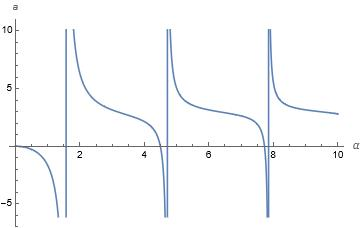
\includegraphics{3d_scattering.jpg}
% \end{figure}

% 可以看到,势$\alpha$随散射长度$a$的变化,当$\alpha_c=(2n+1)\pi/2$时,$a$出现奇异性,对应着束缚态的出现。

% \subsubsection{3D散射中的$\delta$函数}

% 我们首先给出3D散射下散射振幅
% \begin{align}
%    f=\frac{1}{k\mbox{cot}\delta-\mbox{i}k}
% \end{align}
% 观察(\ref{3d_m}),由于$\alpha$是$\mO$(1),因此$a\sim\mO(\Delta)$,因此当势阱宽度趋于0时,散射振幅也趋于0,这种相互作用称为无关相互作用。因此无法用$\delta$函数来模拟球势阱。

% 如果我们用场$\psi$表示散射粒子,拉氏密度为
% \begin{align}
%    \mL = \psi^{\dagger}\Big(\mbox{i}\partial_t+\frac{\nabla^2}{2M}\Big)\psi-\frac{C_0}{4}\Big(\psi^{\dagger}\psi\Big)^2
% \end{align}


\section{介绍}
该章主要参考\cite{scherer2011primer}\cite{郑汉青2019量子场论上}。
\subsection{简介}
首先QCD的拉氏量具有如下形式(仅考虑u、d、s夸克)
\begin{align}
   \mL=\sum_{i=1}^{3}(\bar{q}_i \mbox{i} \slashed{D} q_i-m_i \bar{q}_i q_i)-\frac{1}{4}\mathcal{G}_{\mu \nu}^a \mathcal{G}^{a \mu \nu} 
\end{align}
其中$D_{\mu}=\partial_{\mu}-\mbox{i} g T^a A_{\mu}^a,\ T^a=\lambda^a/2$。仅考虑动能项时,具有$U(3)_L \times U(3)_R$的对称性。量子化之后$U(1)_A$被破坏,系统的对称群为$SU(3)_L \times SU(3)_R \times U(1)_V$,其中$U(1)_V$对应着重子数。由于质量项的存在,$SU(3)_L \times SU(3)_R$遭到了破坏,但当粒子质量相同时,依旧会保持$SU(3)_V$的对称性。

考虑质量项,
\begin{align}
   \sum_{i} m_i \bar{q}_i q_i = \sum_{i,j} \bar{q}_{R,i} M_{ij} q_{L,j}
\end{align}
其中$M=diag(m_u,m_d,m_s)$。如果我们将质量项升级为场,在最后结果的时候在取回常数,并假设其在手征变换下进行如下变换,
\begin{align}\label{rml}
   M \to RML^{\dagger}
\end{align}
则拉氏量依然在$SU(3)_L \times SU(3)_R$变换下不变,由于质量项引起的系统对称性破缺是显式破缺。

但除质量项的显式破缺外,当考虑夸克凝聚的时候,系统也会自发破缺,考虑QCD真空
\begin{align}\label{cds}
   \langle 0 | \bar{q}_{R,i} q_{L,j}| 0 \rangle =\Lambda ^3 \delta_{ij}
\end{align}
其中$\Lambda$具有质量量纲\cite{kaplan2016lectures}。上式在$SU(3)_L \times SU(3)_R$下按照$(3,\bar{3})$变换如下,
\begin{align}
   L_{im}\langle 0 | \bar{q}_{R,n} q_{L,m}| 0 \rangle R^{\dagger}_{nj}=\Lambda ^3 U_{ij}
\end{align}
其中$U_{ij}=(LR^{\dagger})_{ij}$为$SU(3)$中的矩阵。当$L=R$时,$\Sigma_{ij}=\delta_{ij}$,对应真空没有变化,说明QCD凝聚在$SU(3)_V$下不变。当$L\neq R$时,$\Sigma_{ij}$代表此时系统已经变换到了一个和(\ref{cds})不同的真空。如果此时没有质量项的显式破缺,则两个真空简并。

我们可以采用和质量类似的方式,将$U$升级为场,并将其参数化为
\begin{align}
   U(x)=exp[\frac{2\mbox{i} }{f} \phi(x)],\ \phi(x)=T^a \phi^a(x)
\end{align}
其中,$\phi^a(x)$为破缺生成的8个Goldstone玻色子,$T^a$是$SU(3)$群的生成元。

当N=2时,
\begin{align}
   \phi \equiv \sum_{a=1}^{3} \phi_a \sigma^a =
   \begin{pmatrix}
      \phi_3 & \phi_1 - \mbox{i} \phi_2 \\
      \phi_1 + \mbox{i} \phi_2) & -\phi_3
   \end{pmatrix}
   =\begin{pmatrix}
      \pi^0 & \sqrt{2}\pi^+ \\
      \sqrt{2}\pi^- & \pi^0
   \end{pmatrix}
\end{align}

当N=3时,
\begin{align}\label{n3phi}
   \phi \equiv =\sum_{a=1}^{8} \phi_a \lambda^a =
   \begin{pmatrix}
      \pi^0+\frac{\eta}{3} & \sqrt{2}\pi^+ & \sqrt{2}K^+ \\
      \sqrt{2}\pi^- & -\pi^0+\frac{\eta}{3} &\sqrt{2}K^0 \\
      \sqrt{2}K^- & \sqrt{2}\bar{K}^0 & -\frac{2\eta}{3}
   \end{pmatrix}
\end{align}

\subsection{流代数}
   在正式考虑手征拉氏量的写法之前,我们首先讨论与手征相关的流代数。
在手征极限下,拉氏量可以写为
\begin{align}\label{L_QCD}
   \mL_{0} = \sum_{l=u,d,s} (\bar{q}_{R,l} \mbox{i}\slashed{D} q_{R,l} + \bar{q}_{L,l} \mbox{i}\slashed{D} q_{L,l}) -\frac{1}{4}\mathcal{G}_{a\mu\nu}\mathcal{G}_a^{\mu\nu}.
\end{align}
由于上述协变导数是作用到色空间中,因此在$U(3)_L \times U(3)_R$味群作用下保持不变。

考虑整体的$U(3)_L \times U(3)_R$群变换,则场的变化如下
\begin{align*}
   \begin{pmatrix}
      u_L\\
      d_L\\
      s_L
   \end{pmatrix}
   \mapsto U_L
   \begin{pmatrix}
      u_L\\
      d_L\\
      s_L
   \end{pmatrix}
   =
   exp\left(-\mbox{i}\sum_{a=1}^{8}\varepsilon_{La}\frac{\lambda_a}{2}\right)
   e^{-\mbox{i}\varepsilon_L}
   \begin{pmatrix}
      u_L\\
      d_L\\
      s_L
   \end{pmatrix}
\end{align*}

\begin{align}
   \begin{pmatrix}
      u_R\\
      d_R\\
      s_R
   \end{pmatrix}
   \mapsto U_R
   \begin{pmatrix}
      u_R\\
      d_R\\
      s_R
   \end{pmatrix}
   =
   exp\left(-\mbox{i}\sum_{a=1}^{8}\varepsilon_{Ra}\frac{\lambda_a}{2}\right)
   e^{-\mbox{i}\varepsilon_R}
   \begin{pmatrix}
      u_R\\
      d_R\\
      s_R
   \end{pmatrix}
\end{align}
拉氏量的变换为
\begin{align}
   \delta \mL_0 = \bar{q}_R \left(\sum_{a=1}^8\partial_{\mu}\varepsilon_{Ra}\frac{\lambda_a}{2}+\partial_{\mu}\varepsilon_R\right)\gamma^{\mu} q_R + \bar{q}_L \left(\sum_{a=1}^8\partial_{\mu}\varepsilon_{La}\frac{\lambda_a}{2}+\partial_{\mu}\varepsilon_R\right)\gamma^{\mu} q_L
\end{align}
因此产生的左手流和右手流分别为
\begin{align}\label{curr}
   \begin{aligned}
      L^{\mu}_a &= \bar{q}_L\gamma^{\mu}\frac{\lambda_a}{2}q_L, R^{\mu}_a = \bar{q}_R\gamma^{\mu}\frac{\lambda_a}{2}q_R \\
      L^{\mu} &= \bar{q}_L\gamma^{\mu}q_L, R^{\mu} = \bar{q}_R\gamma^{\mu}q_R
   \end{aligned}
\end{align} 
其中带有下指标$a$的流称为八重态,不带有的称为单态。
定义两个单态矢量流和轴矢流为
\begin{align}
   V^{\mu} = R^{\mu} + L^{\mu} = \bar{q}\gamma^{\mu}q, 
   A^{\mu} = R^{\mu} - L^{\mu} = \bar{q}\gamma^{\mu}\gamma_5  q 
\end{align}
定义两个八重态矢量流和轴矢流为
\begin{align}
   V_a^{\mu} = R_a^{\mu} + L_a^{\mu} = \bar{q}\gamma^{\mu}\frac{\lambda_a}{2} q, 
   A_a^{\mu} = R_a^{\mu} - L_a^{\mu} = \bar{q}\gamma^{\mu}\gamma_5 \frac{\lambda_a}{2} q 
\end{align}
单态矢量流即使在量子化之后依旧守恒,对应重子数守恒,而单态轴矢流在考虑量子修正之后出现反常$\partial_{\mu}A^{\mu}=\frac{3g_3^2}{32\pi^2}\epsilon_{\mu\nu\rho\sigma}\mathcal{G}_a^{\mu\nu}\mathcal{G}_a^{\rho\sigma}$。

但是实际的QCD是具有质量项的,因此手征对称性遭到破坏,矢量流和轴矢流在经典情况下也不严格守恒,有
\begin{align}
   \begin{aligned}
   \partial_{\mu} V^{\mu}_a = &\mbox{i}\bar{q}\Big[\mathcal{M},\frac{\lambda_a}{2}\Big]q,\\
   \partial_{\mu} A^{\mu}_a = &\mbox{i}\bar{q}\gamma_5\Big\{\frac{\lambda_a}{2},\mathcal{M}\Big\}q,\\
   \partial_{\mu}V^{\mu}=& 0,\\
   \partial_{\mu}A^{\mu}=&2\mbox{i}\bar{q}\gamma_5\mathcal{M}q,
   \end{aligned}
\end{align}
其中$\mathcal{M}=diag\{m_u,m_d,m_s\}$为质量矩阵。可以看出,如果三种夸克质量一样,则质量矩阵为单位矩阵,矢量流严格守恒。如果质量矩阵很小,矢量流和轴矢流也近似守恒。由于u、d夸克质量相近,且远小于s夸克质量,因此$SU(2)_L\times SU(2)_R$群对称性就比$SU(3)_L\times SU(3)_R$对称性要好很多。

根据(\ref{curr})定义三个荷算符:
\begin{align}
   \begin{aligned}
      Q_{La}(t) &= \int \mbox{d}^3x q_L^{\dagger}(t,\vec{x}) \frac{\lambda_a}{2}q_L(t,\vec{x})\\
      Q_{Ra}(t) &= \int \mbox{d}^3x q_R^{\dagger}(t,\vec{x}) \frac{\lambda_a}{2}q_R(t,\vec{x})\\
      Q_{V}(t) &= \int \mbox{d}^3x q^{\dagger}(t,\vec{x}) q(t,\vec{x})
   \end{aligned}   
\end{align}
三个荷算符之间的对易关系恰好对应着$SU(3)_L\times SU(3)_R\times U(1)_V$的李代数
\begin{align}
   \begin{aligned}
      [Q_{La},Q_{Lb}]=\mbox{i}f_{abc}Q_{Lc}, [Q_{Ra},Q_{Rb}]=\mbox{i}f_{abc}Q_{Rc}\\
      [Q_{La},Q_{Rb}]=[Q_{La},Q_V]=[Q_{Ra},Q_V]=0
   \end{aligned}
\end{align}

验证第一个对易关系:
\begin{align*}
   [Q_{La},Q_{Lb}] =& \int \mbox{d}^3x \mbox{d}^3y \Bigl[q_L^{\dagger}(t,\vec{x})\frac{\lambda^a}{2}q_L(t,\vec{x}),q_L^{\dagger}(t,\vec{y})\frac{\lambda^a}{2}q_L(t,\vec{y})\Bigr] \\
   =&\int \mbox{d}^3x \mbox{d}^3y \Bigl[q^{\dagger}(t,\vec{x})P_L\frac{\lambda^a}{2}q(t,\vec{x}),q^{\dagger}(t,\vec{y})P_L\frac{\lambda^a}{2}q(t,\vec{y}\Bigr])\\
   =&\int \mbox{d}^3x \mbox{d}^3y \delta^3(\vec{x}-\vec{y})q^{\dagger}(t,\vec{x})P_L\frac{\lambda_a}{2}\frac{\lambda_b}{2}q(t,\vec{y})\\
   &-\int \mbox{d}^3x \mbox{d}^3y \delta^3(\vec{x}-\vec{y})q^{\dagger}(t,\vec{y})P_L\frac{\lambda_a}{2}\frac{\lambda_b}{2}q(t,\vec{x})\\
   =& \mbox{i}f_{abc}\int \mbox{d}^3xq^{\dagger}(t,\vec{x})P_L\frac{\lambda_c}{2}q(t,\vec{x})=\mbox{i}f_{abc}Q^{Lc}
\end{align*}

除此之外,还可以得到流之间的对易关系如下:
\begin{align}
   \begin{aligned}
   [V^0_a(t,\vec{x}),V^{\mu}_b(t,\vec{y})] =& \delta^3(\vec{x}-\vec{y})\mbox{i}f_{abc}V^{\mu}_c(t,\vec{X}),\\
   [V^0_a(t,\vec{x}),V^{\mu}(t,\vec{y})] =& 0,\\
   [V^0_a(t,\vec{x}),A^{\mu}_b(t,\vec{y})] =& \delta^3(\vec{x}-\vec{y})\mbox{i}f_{abc}A^{\mu}_c(t,\vec{X}),\\
   [A^0_a(t,\vec{x}),V^{\mu}_b(t,\vec{y})] =& \delta^3(\vec{x}-\vec{y})\mbox{i}f_{abc}A^{\mu}_c(t,\vec{X}),\\
   [A^0_a(t,\vec{x}),V^{\mu}(t,\vec{y})] =& 0,\\
   [A^0_a(t,\vec{x}),A^{\mu}_b(t,\vec{y})] =& \delta^3(\vec{x}-\vec{y})\mbox{i}f_{abc}V^{\mu}_c(t,\vec{X}).\\
   \end{aligned}
\end{align}

% \subsection{对称性的破缺}

% \subsection{Goldstone玻色子的实现}
% 在手征极限下,系统拉氏量(\ref*{L_QCD})具有$SU(3)_L\times SU(3)_R \times U(1)_V$的对称性,但当考虑夸克凝聚的时候,基态只有$SU(3)_V \times U(1)_V$的对称性,系统的对称性发生了自发破缺,生成了8个无质量的Goldstone玻色子。由于真实的夸克带有微小质量,因此拉氏量不具备严格的$SU(3)_L\times SU(3)_R \times U(1)_V$的对称性,破缺得到的Goldstone玻色子带有质量。

% 一般考虑,假设有大群G,以及它的子群H,拉氏量具有群G对称性,基态具有群H对称性,则会生成$n=n_G-n_H$个Goldstone玻色子,每个Goldstone玻色子用$\phi_i$标记,为光滑实函数,$i=1,...,n$,定义一个n分量的矢量$\bm{\Phi}=(\phi_1,...,\phi_n)$,接着定义一个实向量空间
% \begin{align}
%    M_1 = \{\bm{\Phi}:M^4 \to \mathbb{R^n}| \phi_i: M^4\to R\}
% \end{align}
% 定义一个映射$\varphi : G \times M_1 \to M_1$,满足
% \begin{itemize}
%    \item 
%    $\varphi(e,\bm{\Phi})=\bm{\Phi}$
%    \item 
%    $\varphi(g_1,\varphi(g_2,\bm{\Phi}))=\varphi(g_1 g_2 ,\bm{\Phi})$
% \end{itemize}
% 用\bm{\Phi}表示$M_1$中的原点,\textcolor{blue}{对应系统的基态构型},则对于$\forall h \in H$,存在$\varphi(h,0)=0$,从而可以建立起$G/H$陪集与Goldstone玻色子之间的同构关系。可以验证,对于同一陪集中的元素,原点被映射到同一矢量,而不同陪集中的元素将原点映射到不同矢量。

% 考查Goldstone玻色子在群G下的变换行为,对于每一个$\bm{\Phi}$有一个陪集$\tilde{g}H$与之对应,表示为
% \begin{align*}
%    \varphi(g,\bm{\Phi})=\varphi(\tilde{g}h,0)
% \end{align*}
% 接着用$\varphi(g)$作用到$\bm{\Phi}$上
% \begin{align*}
%    \varphi(g,\bm{\Phi})=\varphi(g,\varphi(\tilde{g}h,0))=\bm{\Phi}^{\prime}
% \end{align*}
% 即存在关系
% \begin{center}
% \begin{math}
%    \begin{aligned}
%       \bm{\Phi} &\stackrel{g}{\longrightarrow} &\bm{\Phi}^{\prime}\\
%       \downarrow &&\uparrow\\
%       \tilde{g}H &\stackrel{g}{\longrightarrow}& g \tilde{g}H
%    \end{aligned}
% \end{math}
% \end{center}

% % \section{线性$\sigma$ 模型}
% % 线性$\sigma$模型的拉氏量如下
% % \begin{align}
% %    \mL = 
% % \end{align}

\newpage

\section{介子的手征拉氏量}
\subsection{手征的power-counting}
手征拉氏量一般具有如下形式
\begin{align}
   \mL_{\text{eff}} = \mL_2 + \mL_4 + \mL_6+\cdots,
\end{align}
其中只包含偶数项。这主要是由于Lorentz不变性以及质量项是$\sim\mO(q^2)$的。

对于给定费曼图,在$p_i \mapsto t p_i$以及$m_q \mapsto t^2 m_q$变换下,若不变振幅变换如下
\begin{align}
   M(tp_i,t^2m_q) = t^D M(p_i,m_q),
\end{align}
则称D是一个图的手征阶数。手征阶数的计算公式如下
\begin{align}
   D = nN_L-2N_I + \sum_{k=1}^{\infty} 2k N_{2k},
\end{align}
其来源简单阐述如下,在上述标度变化下,传播子的变换如下
\begin{align}
   \begin{aligned}
      \int \frac{\mbox{d}^nk}{(2\pi)^n}\frac{\mbox{i}}{k^2-M^2+\mbox{i}\epsilon} 
      \mapsto& \int \frac{\mbox{d}^nk}{(2\pi)^n}\frac{\mbox{i}}{t^2(k^2/t^2-M^2+\mbox{i}\epsilon)}\\
      \stackrel{k=tk^{\prime}}{=}& t^{n-2}\int \frac{\mbox{d}^n k^{\prime}}{(2\pi)^n}\frac{\mbox{i}}{k^{\prime 2}-M^2+\mbox{i}\epsilon},
   \end{aligned}
\end{align}
因此内线的变换为$t^{n-2}$,而顶点的变换为
\begin{align}
   \delta^n(q)q^{2k} \mapsto t^{2k-n}\delta^n{q}q^{2k},
\end{align}
因此内线的变化为$t^{2k-n}$,此外由于散射矩阵的不变性,以及$S\sim\delta^n(q)M$,因此需要加上一个$n$来补偿$\delta$函数的影响,此时我们可以得到
\begin{align}
   D = n + (n-2)N_I + \sum_{k=1}^{\infty} N_{2k}(2k-n).
\end{align}
再考虑到一张图中独立圈数、内线数、顶点数之间的关系$N_L = N_I - (N_V - 1)$,其中$N_V=\sum_{k=1}^{\infty}N_{2k}$,即可得到上式。

\subsection{外源}
该章主要参考\cite{scherer2011primer}。

通常在量子场论中,紫外的微观理论与红外的理论可以截然不同,如QCD。低能有效作用量是通过积掉一些高能的自由度来得到的。但是在实际操作中很难实行,我们往往首先猜测红外的场以及可能的对称性,然后写下与对称性自洽的有效有效作用,最后再在实验中进行检验。

首先考虑QCD的拉氏量如下,
\begin{align}
   \mL_{QCD}^0=\sum_{i=1}^{3}\bar{q}_i \mbox{i} \slashed{D} q_i-\frac{1}{4}\mathcal{G}_{\mu \nu}^a \mathcal{G}^{a \mu \nu},
\end{align}
上述拉氏量具有$SU(3)_L\times SU(3)_R$的味道对称性,如果想要引入局域的味道空间的变换,我们需要引入以下外源(类似于规范理论中的规范场)\cite{GASSER1984142}\cite{GASSER1985465},
\begin{align}
   \mL = \mL_{QCD}^0 + \mL_{ext},
\end{align}
其中
\begin{align}
   \begin{aligned}
   \mL_{ext} =& \sum_{a=1}^8 v_a^{\mu} \bar{q} \gamma_{\mu}\frac{\lambda_a}{2}q + v_{(s)}^{\mu}\frac{1}{3}\bar{q}\gamma_{\mu}q + \sum_{a=1}^8 a_{a}^{\mu} \bar{q} \gamma_{\mu} \gamma_5 \frac{\lambda_a}{2}q\\
   &-\sum_{a=0}^{8}s_{a}\bar{q}\lambda_{a}q + \sum_{a=0}^{8}p_{a}\mbox{i}\bar{q}\gamma_5 \lambda_a q\\
   =&\bar{q}\gamma_{\mu}\Bigl(v^{\mu}+\frac{1}{3}v_{(s)}^{\mu}+\gamma_5 a^{\mu}\Bigr)q -\bar{q}(s-\mbox{i}\gamma_5 p)q,
   \end{aligned}
\end{align}
其中
\begin{align}
   v_{\mu} = v_{\mu}^a\frac{\lambda_a}{2},a_{\mu} = a_{\mu}^a\frac{\lambda_a}{2},s_{\mu} = s_{\mu}^a\frac{\lambda_a}{2},p_{\mu} = p_{\mu}^a\frac{\lambda_a}{2},
\end{align}
分别是引入的矢量、轴矢量、标量和赝标量外场。当我们取外源$v^{\mu}=v_{(s)}^{\mu}=a^{\mu}=p=0$以及$s=diag(m_u,m_d,m_s)$是,上述拉氏量回到原始QCD拉氏量。

我们可以将上述拉氏量通过手征投影算符改写为
\begin{align}
   \begin{aligned}
   \mL =& \mL_{QCD}^0 + \bar{q}_L\gamma^{\mu}\Bigl(l_{\mu}+\frac{1}{3}v_{\mu}^{(s)}\Bigr)q_L + \bar{q}_R\gamma_{\mu}\Bigl(r_{\mu}+\frac{1}{3}v_{\mu}^{(s)}\Bigr)\\
   & -\bar{q}_R(s+\mbox{i}p)q_L - \bar{q}_L(s-\mbox{i}p)q_R,
   \end{aligned}
\end{align}
其中$r_{\mu}=v_{\mu}+a_{\mu},l_{\mu}=v_{\mu}-a_{\mu}$。如果想要上述拉氏量在$SU(3)_L\times SU(3)_R$下保持不变,即
\begin{align}
   \begin{aligned}
   q_R &\mapsto V_R(x)q_R\\
   q_L &\mapsto V_L(x)q_L,
   \end{aligned}
\end{align}
则需要外场作如下变换
\begin{align}
   \begin{aligned}
   r_{\mu} &\mapsto V_R r_{\mu} V_R^{\dagger} + \mbox{i} V_R \partial_{\mu} V_R^{\dagger},\\
   l_{\mu} &\mapsto V_L l_{\mu} V_L^{\dagger} + \mbox{i} V_L \partial_{\mu} V_L^{\dagger},\\
   v_{\mu}^{(s)} &\mapsto v_{\mu}  - \partial_{\mu} \Theta,\\
   s + \mbox{i}p &\mapsto V_R(s+\mbox{i}p)V_L^{\dagger},\\
   s - \mbox{i}p &\mapsto V_L(s-\mbox{i}p)V_R^{\dagger}.
   \end{aligned}
\end{align}
除了要求拉氏量在上述局域$SU(3)_L\times SU(3)_R$下保持不变之外,我们还要求拉氏量能够满足C、P、T对称。由于CPT定理的存在,因此我们可以只考虑C、P变换下上述外场的变换情况。

在P变换下,夸克场和拉氏量的变换为
\begin{align}
   q_f(t,\vec{x})\stackrel{P}{\mapsto} \gamma_0 q_f(t,-\vec{x}), \mL(t,\vec{x}) \stackrel{P}{\mapsto} \mL(t,-\vec{x}),
\end{align}
因此外场的变换为
\begin{align}
   v^{\mu}\stackrel{P}{\mapsto} v_{\mu},v_{(s)}^{\mu}\stackrel{P}{\mapsto} v^{(s)}_{\mu},a^{\mu}\stackrel{P}{\mapsto} -a_{\mu},s\stackrel{P}{\mapsto} s,p\stackrel{P}{\mapsto}-p.
\end{align}
同理可得C变换下外场的变换为
\begin{align}
   v_{\mu}\stackrel{C}{\mapsto} -v^T_{\mu},v^{(s)}_{\mu}\stackrel{C}{\mapsto} -v^{(s)T}_{\mu},a_{\mu}\stackrel{C}{\mapsto} a^T_{\mu},s\stackrel{C}{\mapsto} s^T,p\stackrel{C}{\mapsto}p^T.
\end{align}

考虑一个简单的例子,QED是U(1)规范理论,而U(1)群是$SU(3)_L\times SU(3)_R$的子群。我们可以令
\begin{align}
   r_{\mu} = l_{\mu} = -e \mathcal{A}_{\mu} Q,
\end{align}
其中$Q=diag(2/3,-1/3,-1/3)$,此时可以得到
\begin{align}
   \begin{aligned}
      \mL_{\text{ext}} &= -e\mathcal{A}_{\mu}(\bar{q}_L Q \gamma_{\mu} q_L + \bar{q}_R Q \gamma_{\mu}q_R)=-e\mathcal{A}_{\mu}\bar{q}Q\gamma_{\mu}q\\
      &=-e\mathcal{A}_{\mu}\Bigl(\frac{2}{3}\bar{u}\gamma_{\mu}u-\frac{1}{3}\bar{d}\gamma_{\mu}d-\frac{1}{3}\bar{s}\gamma_{\mu}s\Bigr)=-e\mathcal{A}_{\mu} J^{\mu},
   \end{aligned}
\end{align}
即光子场和夸克场的耦合。

\subsection{两个常数}
首先我们已经将破缺的8个Goldstone玻色子参数化为
\begin{align}
   U(x) = \text{exp}\Bigl(\frac{\mbox{i}\phi(x)}{F_0}\Bigr),
\end{align}
其中$\phi$取自(\ref{n3phi})式,$F_0$为手征极限下$\pi$介子的真空衰变常数,带有质量量纲。$U$在$SU(3)_L\times SU(3)_R$群下的变换方式为
\begin{align}
   U(x) \mapsto RU(x)L^{\dagger}.
\end{align}

此时,我们能写下的包含最少导数且保证手征不变的拉氏量为
\begin{align}
   \mL_{\text{eff}}=\frac{F_0^2}{4}\text{Tr}(\partial_{\mu}U\partial^{\mu}U^{\dagger}).
\end{align}
考虑无穷小的$SU(3)_L$变换,可以得到左手流为
\begin{align}
   J^{\mu}_{La}=\mbox{i}\frac{F_0^2}{4}\text{Tr}(\lambda_a\partial^{\mu}U^{\dagger}U),
\end{align}
同理可得右手流为
\begin{align}
   J^{\mu}_{Ra}=-\mbox{i}\frac{F_0^2}{4}\text{Tr}(\lambda_aU\partial^{\mu}U^{\dagger}).
\end{align}

定义矢量流和轴矢流分别为
\begin{align}
   J_{Va}^{\mu}=&J_{Ra}^{\mu}+J_{La}^{\mu}=-\mbox{i}\frac{F_0^2}{4}\text{Tr}(\lambda_a[U,\partial^{\mu}U^{\dagger}]),\\
   J_{Aa}^{\mu}=&J_{Ra}^{\mu}-J_{La}^{\mu}=-\mbox{i}\frac{F_0^2}{4}\text{Tr}(\lambda_a\{U,\partial^{\mu}U^{\dagger}\}).
\end{align}
将$U$做泰勒展开,我们可以得到轴矢流最低阶为
\begin{align}
   J^{\mu}_{Aa}=-F_0\partial^{\mu}\phi_a+\cdots,
\end{align}
此时我们可以计算轴矢流在Goldstone玻色子和真空态之间的矩阵元为
\begin{align}
   \langle 0|J^{\mu}_{Aa}(x)|\phi_b(p)\rangle = \langle 0|-F_0 \partial^{\mu}\phi_a(x)|\phi_b(x)\rangle=\mbox{i}p^{\mu}F_0\text{exp}(-\mbox{i}p \cdot x)\delta_{ab},
\end{align}
从中我们可以看到$F_0$的物理意义。

严格的对称性破缺我们可以得到严格的零质量Goldstone玻色子,但是通过实验我们知道$\pi,K$等介子是有质量的,因此我们必须引入QCD中显式的质量破缺项,且假设质量矩阵按照(\ref{rml})进行变换。则此时我们能写下的拉氏量为
\begin{align}
   \mL_{\text{s.b.}}=\frac{F_0^2B_0}{2}\text{Tr}(\mathcal{M}U^{\dagger}+U\mathcal{M^{\dagger}}),
\end{align}
其中下标$\text{s.b.}$代表对称性破缺。通过比较其基态能量密度关于夸克质量的导数和QCD中相应量
\begin{align}
   \langle \mathcal{H}_{\text{eff}}\rangle_{min}=-F_0^2B_0(m_u+m_d+m_s),\\
   \frac{\partial\langle 0|\mathcal{H}_{\text{QCD}}|0\rangle}{\partial m_q}\Big|_{m_u=m_d=m_s=0}=\frac{1}{3}\langle\bar{q}q\rangle_0
\end{align}
可得,
\begin{align}
   3F_0^2B_0=-\langle\bar{q}q\rangle_0,
\end{align}
即$B_0$与标量单态夸克凝聚有关。

接着将$U$进行泰勒展开,我们可以得到
\begin{align}
   \mathcal{L}_{\text{s.b.}} = -\frac{B_0}{2}\text{Tr}(\phi^2\mathcal{M})+\cdots
\end{align}
代入(\ref{n3phi})式,我们可以得到
\begin{align}
   \begin{aligned}
   \text{Tr}(\phi^2\mathcal{M})=&2(m_u+m_d)\pi^{+}\pi^{-}+2(m_u+m_s)K^{+}K^{-}+2(m_d+m_s)K^0\bar{K}^0\\
   &+(m_u+m_d)\pi^0\pi^0+\frac{2}{\sqrt{3}}(m_u-m_d)\pi^0\eta+\frac{m_u+m_d+4m_s}{3}\eta^2.
   \end{aligned}
\end{align}
为简单起见,令$m_u=m_d=\hat{m}$,因此我们可以得到在最低阶Goldstone玻色子质量和夸克质量的关系
\begin{align}
   M_{\pi}^2=&2B_0\hat{m},\\
   M_k^2=&B_0(\hat{m}+m_s),\\
   M_{\eta}^2=&\frac{2}{3}B_0(\hat{m}+2m_s).
\end{align}
此时我们可以得到著名的Gell-Mann-Okubo关系:
\begin{align}
   4M_K^2=3M_{\eta}^2+M_{\pi}^2.
\end{align}







\subsection{最低阶手征拉氏量}
有了上面的准备之后,我们就可以开始构造手征拉氏量了。

首先,我们需要定义场算符的协变导数,以场算符$A$为例,协变导数为
\begin{align}
   D_{\mu}A=\partial_{\mu}A-\mbox{i}r_{\mu}A+\mbox{i}Al_{\mu}.
\end{align}
可以验证,协变导数在$SU(3)_L\times SU(3)_R$群下的变换方式为
\begin{align}
   D_{\mu}A \mapsto R(D_{\mu}A)L^{\dagger}.
\end{align}
由于有效拉氏量中会包含任意高阶的导数项,因此我们还需要引入外场的场强张量
\begin{align}
   f_{R\mu\nu}=&\partial_{\mu}r_{\nu}-\partial_{\nu}r_{\mu}-\mbox{i}[r_{\mu},r_{\nu}],\\
   f_{L\mu\nu}=&\partial_{\mu}l_{\nu}-\partial_{\nu}l_{\mu}-\mbox{i}[l_{\mu},l_{\nu}].
\end{align}
接着我们定义一个标量和赝标量外场的线性组合项$\chi=2B_0(s+\mbox{i}p)$。

由于手征拉氏量是按照外动量阶数展开的,因此我们需要知道它们关于外动量的阶数,如下所示,
\begin{align}
   U=\mathcal{O}(q^0),D_{\mu}U=\mathcal{O}(q),r_{\mu},l_{\mu}=\mO (q), f_{L,R \mu \nu}=\mO(q^2), \chi = \mO (q^2),
\end{align}
因此可以写出满足对称性要求的二阶的手征拉式量如下\cite{GASSER1985465},
\begin{align}
   \mL_2 =\frac{F_0^2}{4} \text{Tr}[D_{\mu}U (D^{\mu}U)^{\dagger}] + \frac{F_0^2}{4} \text{Tr}[\chi U^{\dagger} + U \chi^{\dagger}],
\end{align}
在这里我们舍弃了不满足$P$宇称的$\text{Tr}[\chi U^{\dagger}-U\chi^{\dagger}]$项,其中包含两个低能常数$F_0$和$B_0$。

\subsection{$\pi-\pi$散射的例子}
考虑一个$SU(2)_L\times SU(2)_R$的二阶拉氏量,即$m_u=m_d=0$,而$m_s$依旧取其物理值,且令$r_{\mu}=l_{\mu}=0$,
\begin{align}
   \mL_2 = \frac{F^2}{4}\text{Tr}(\partial_{\mu}U\partial^{\mu}U^{\dagger})+\frac{F^2}{4}\text{Tr}(\chi U^{\dagger}+U\chi^{\dagger}),
\end{align}
其中
\begin{align*}
   \chi = 2B\mathcal{M} = &2B
   \begin{pmatrix}
      \hat{m} & 0\\
      0 & \hat{m}
   \end{pmatrix},\\
U=\text{exp}\Bigl(\mbox{i}\frac{\phi}{F}\Bigr),
\phi =& \sum_{i=1}^3 \phi_i \tau_i =
\begin{pmatrix}
   \pi^0 & \sqrt{2}\pi^{+}\\
   \sqrt{2}\phi^{-} & -\pi^0
\end{pmatrix},
\end{align*}
不带有下标0的$F$和$B$表示我们此时考虑的对称性是$SU(2)_L\times SU(2)_R$。我们将
\begin{align}
   U = 1 +\mbox{i}\frac{\phi}{F}-\frac{1}{2}\frac{\phi^2}{F^2}-\frac{\mbox{i}}{6}\frac{\phi^3}{F^3}+\frac{1}{24}\frac{\phi^4}{F^4}+\cdots
\end{align}
代入,可得
\begin{align}
   \mL_2 =\mL_2^{2\phi}+\mL_2^{4\phi}+\cdots, 
\end{align}
因为$\mL$不包含三点相互作用,因此最低阶相互作用项为
\begin{align}
   \mL_2^{4\phi}=\frac{1}{6F^2}(\phi_i\partial^{\mu}\phi_i\partial_{\mu}\phi_j\phi_j-\phi_i\phi_i\partial_{\mu}\phi_j\partial^{\mu}\phi_j)+\frac{M^2}{24F^2}\phi_i\phi_i\phi_j\phi_j,
\end{align}
其中$M^2=2B\hat{m}$。

我们可以计算上述相互作用项的矩阵元,例如
\begin{align}
   \langle p_c,c;p_d,d|\phi_i\partial^{\mu}\phi_i\partial_{\mu}\phi_j\phi_j|p_a,a;p_b,b\rangle
\end{align}
的收缩方式共24种,以其中一种为例
\begin{align*}
   \begin{aligned}
   \bcontraction[1ex]{p}{_c}{,c;p_d,d|\phi}{_i}
   \bcontraction[1ex]{p_c,c;p_d,d|\phi_i\partial^{\mu}\phi_i\partial_{\mu}}{\phi}{_j\phi_j|p}{_a}
   \bcontraction[2ex]{p_c,c;p}{_d}{,d|\phi_i\partial^{\mu}}{\phi}
   \bcontraction[2ex]{p_c,c;p_d,d|\phi_i\partial^{\mu}\phi_i\partial_{\mu}\phi_j\phi}{_j}{|p_a,a;p}{_b}
   \langle p_c,c;p_d,d|\phi_i\partial^{\mu}\phi_i\partial_{\mu}\phi_j\phi_j|p_a,a;p_b,b\rangle\\
   \Rightarrow \delta_{ic}\mbox{i}p_{d}^{\mu}\delta_{id}(-\mbox{i}p_{a\mu}\delta_{ja}\delta_{jb})=
   p_a \cdot p_d \delta_{ab}\delta_{cd}
   \end{aligned}
\end{align*}
因此对应如图\ref{pipi}所示的费曼图,可以得到其散射振幅为
\begin{figure}
   \centering
   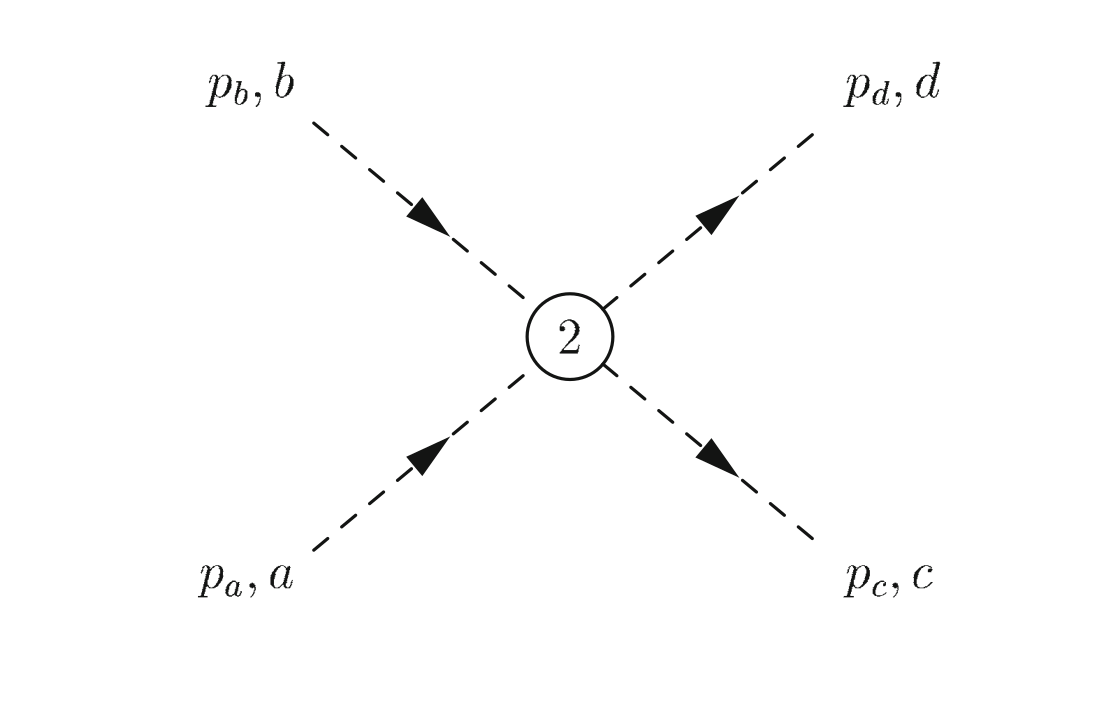
\includegraphics[scale=0.4]{l2pipi.png}
   \caption{最低阶$\pi\pi$散射}\label{pipi}
\end{figure}

\begin{align}\label{mpipi}
   \begin{aligned}
   \mathcal{M} =& \mbox{i}\Bigl[\delta_{ab}\delta_{cd}\frac{s-M^2}{F^2}+\delta_{ac}\delta_{bd}\frac{t-M^2}{F^2}+\delta_{ad}\delta_{bc}\frac{u-M^2}{F^2}\Bigr]
   \\
   & - \frac{\mbox{i}}{3F^2}(\delta_{ab}\delta_{cd}+\delta_{ac}\delta_{bd}+\delta_{ad}\delta_{bc})(\Lambda_a+\Lambda_b+\Lambda_c+\Lambda_d),
\end{aligned}
\end{align}
其中$\Lambda_k=p_k^2-M^2$。
通常对于$\pi_a(p_a)+\pi_b(p_b)\to \pi_c(p_c)+\pi_d(p_d)$过程的$T$矩阵($\mathcal{M}=\mbox{i}T$)可以参数化为
\begin{align}\label{tpipi}
   T_{ab;cd}(p_a,p_b;p_c,p_d)=\delta_{ab}\delta_{cd}A(s,t,u)+\delta_{ac}\delta_{bd}A(t,s,t)+\delta_{ad}\delta_{bc}A(u,t,s)。
\end{align}
其中$A(s,t,u)=A(s,u,t)$。可以看出在$\mathcal{O}(q^2)$阶,
\begin{align}
   A(s,t,u)=\frac{s-M^2}{F^2}.
\end{align}



除了手征之外,我们还通常利用同位旋对称性来研究$\pi\pi$散射,在$SU(2)$极限下,$\pi$介子组成同位旋三重态,因此强相互作用是同位旋不变的。对于$T$矩阵,我们可以写出
\begin{align}
   \langle I^{\prime},I^{\prime}_3|T|I,I_3\rangle = T^I \delta_{II^{\prime}}\delta_{I_3I_3^{\prime}}。
\end{align}
因此$\pi\pi$散射的同位旋振幅可以根据(\ref{tpipi})式拆解为\cite{GASSER1984142}
\begin{align}
   \begin{aligned}
   T^{I=0}&=3A(s,t,u)+A(t,u,s)+A(u,s,t),\\
   T^{I=1}&=A(s,t,u)-A(u,s,t),\\
   T^{I=2}&=A(t,u,s)+A(u,s,t).
   \end{aligned}
\end{align}
计算开启域附近的$T$矩阵,我们可以得到s波的散射长度
\begin{align}\label{a}
   T^{I=0}|_{\text{thr}} = 32\pi a_0^0,\ T^{I=2}|_{\text{thr}}=32\pi a_0^2,
\end{align}
其中$a$的上标代表同位旋,下标代表s波散射。由于玻色对称性,$T^{I=1}=0$。结合手征理论,我们可以得到两个散射长度的值。

首先,我们有
\begin{align}
   A(s_{\text{thr}},t_{\text{thr}},u_{\text{thr}})=\frac{3M_{\pi}^2}{F_{\pi}^2},
\end{align}
其中$F_{\pi}$、$M_{\pi}$和$F$、$M$的区别仅在$\mathcal{Q}(p^4)$开始显现。在这里,我们先用带有下标的表示。
因此,对于不同的同位旋振幅我们有
\begin{itemize}
 
\item I=0:
\begin{align}
   \begin{aligned}
   T^{I=0}|_{\text{thr}}=&[3A(s,t,u)+A(t,u,s)+A(u,s,t)]|_{\text{thr}}\\
   =&[2A(s,t,u)+A(s,t,u)+A(t,u,s)+A(u,s,t)]|_{\text{thr}}\\
   =&\frac{6M_{\pi}^2}{F_{\pi}^2}+\frac{[s+t+u-3M_{\pi}^2]|_{\text{thr}}}{F_{\pi}^2}\\
   =&\frac{7M_{\pi}^2}{F_{\pi}^2}.
   \end{aligned}
\end{align}
\item I=2:
\begin{align}
   \begin{aligned}
   T^{I=2}|_{\text{thr}}=&[A(t,u,s)+A(u,s,t)]|_{\text{thr}}\\
   =&[A(t,u,s)+A(u,s,t)+A(s,t,u)-A(s,t,u)]|_{\text{thr}}\\
   =&\frac{M_{\pi}^2}{F_{\pi}^2}-\frac{3M_{\pi}^2}{F_{\pi}^2}\\
   =&-\frac{2M_{\pi}^2}{F_{\pi}^2}.
\end{aligned}
\end{align}
代回(\ref{a})式,我们可以得到
\begin{align}
   a_0^0=\frac{7M_{\pi}^2}{32F_{\pi}^2}=0.159,\ a_0^2 = -\frac{M_{\pi}^2}{16\pi F_{\pi}^2}=-0.0454,
\end{align}
在这里我们代入了$F_{\pi}=92.4\text{MeV}$和$M_{\pi}=M_{\pi^+}=139.57\text{MeV}$。

\end{itemize}

\subsection{超出领头阶}
我们在这里直接给出$\mathcal{O}(q^4)$的拉氏量\cite{GASSER1985465}
\begin{align}
   \begin{aligned}
      \mL_4 = &L_1\Bigl\{\text{Tr}[D_{\mu}U(D^{\mu}U)^{\dagger}]\Bigr\}^2+L_2\text{Tr}[D_{\mu}(D_{\nu}U)^{\dagger}]\Tr[D^{\mu}U(D^{\nu})^{\dagger}]\\
      & +L_3\Tr[D_{\mu}U(D^{\mu}U)^{\dagger}D_{\nu}U(D^{\nu}U)^{\dagger}]+L_4\Tr[D_{\mu}U(D^{\mu}U)^{\dagger}]\Tr(\chi U^{\dagger}+U\chi^{\dagger})\\
      & +L_5\Tr[D_{\mu}U(D^{\mu}U)^{\dagger}(\chi U^{\dagger}+U\chi^{\dagger})]+L_6[\Tr(\chi U^{\dagger}+U\chi^{\dagger})]^2\\
      & +L_7[\Tr(\chi U^{\dagger}-U\chi^{\dagger})]^2+L_8\Tr(U\chi^{\dagger}U\chi^{\dagger}+\chi U^{\dagger}\chi U^{\dagger})\\
      & -\mbox{i}L_9\Tr[f_{\mu\nu}^R D^{\mu}U(D^{\nu}U)^{\dagger}+f_{\mu\nu}^L (D^{\mu}U)^{\dagger}D^{\nu}U]+L_{10}\Tr(Uf_{\mu\nu}^L U^{\dagger}f^{\mu\nu}_R)\\
      & +H_1\Tr(f_{\mu\nu}^Rf_R^{\mu\nu}+f_{\mu\nu}^Lf_L^{\mu\nu})+H_2\Tr(\chi\chi^{\dagger}).
   \end{aligned}
\end{align}
这里每项前面的系数同$F_0$和$B_0$一样,目前没法通过理论决定,只能由实验给出。

\textbf{$\mathcal{O}(q^4)$阶的Goldstone玻色子的质量}

为了计算Goldstone玻色子的自能,在这里我们忽略外场,且假设$m_u=m_d=\hat{m}$,$m_s$取其物理质量。首先,最低阶拉氏量给出的费曼传播子为
\begin{align}
   \Delta_{F\phi}(p)=\frac{1}{p^2-M_{\phi,2}^2}+\mbox{i}\epsilon,\ \phi = \pi,K,\eta,
\end{align}
其中$M_{\pi,2}^2=2B_0\hat{m},M_{K,2}^2=B_0(\hat{m}+m_s),M_{\eta,2}^2=\frac{2}{3}B_0(\hat{m}+2m_s)$,下标2表示手征二阶给出的结果。用$-\mbox{i}\Sigma_{\phi}(p^2)$代表单粒子不可约图,则完整的传播子为
\begin{align}
   \begin{aligned}
   \mbox{i}\Delta_{\phi}(p)&=\frac{\mbox{i}}{p^2-M^{2}_{\phi,2}+\mbox{i}\epsilon}+\frac{\mbox{i}}{p^2-M^{2}_{\phi,2}+\mbox{i}\epsilon}[-\mbox{i}\Sigma_{\phi}(p^2)]\frac{\mbox{i}}{p^2-M^{2}_{\phi,2}+\mbox{i}\epsilon}+\cdots\\
   &=\frac{\mbox{i}}{p^2-M^{2}_{\phi,2}-\Sigma_{\phi}(p^2)+\mbox{i}\epsilon}.
   \end{aligned}
\end{align}
物理质量定义在传播子的极点处
\begin{align}
   M_{\phi}^2 -M_{\phi,2}^2-\Sigma_{\phi}(M_{\phi}^2)=0
\end{align}

$\mathcal{O}(q^4)$阶的自能图如图\ref{zineng}所示,
\begin{figure}
   \centering
   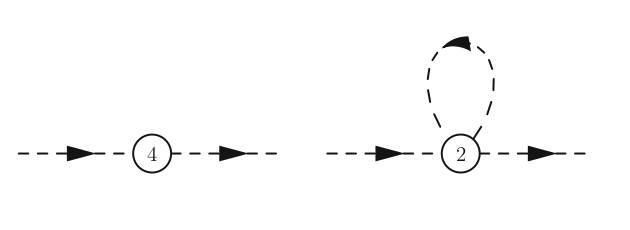
\includegraphics[scale=0.7]{4zineng.png}\caption{$\mathcal{O}(q^4)$阶的自能图}\label{zineng}
\end{figure}
由图可以看出,我们需要的相互作用拉氏量应具有如下形式
\begin{align}
   \mL_{\text{int}}=\mL_2^{4\phi}+\mL_4^{2\phi},
\end{align}
其中的$\mL_2^{4\phi}$仿照$\pi\pi$散射的例子可以给出如下
\begin{align}
   \mL_2^{4\phi}=\frac{1}{48F_0^2}\Bigl\{\Tr([\phi,\partial_{\mu}\phi][\phi,\partial^{\mu}\phi])+2B_0\Tr(\mathcal{M}\phi^4)\Bigr\}
\end{align}

观察$\mL_4^{2\phi}$可以发现,由于外场等于0,因此其中正比于$L_9,L_{10},H_1,H_2$的项没有贡献。此外,$L_1,L_2,L_3$的项都是$\mathcal{O}(\phi^4)$的,不需要考虑。因此对于$\mL_4^{2\phi}$有贡献的只能$L_4-L_8$项。以$L_4$为例,
\begin{align}
   \begin{aligned}
      L_4\Tr[D_{\mu}U(D^{\mu}U)^{\dagger}]\Tr(\chi U^{\dagger}+U\chi^{\dagger}) =& L_4\frac{2}{F_0^2}[\partial_{\mu}\eta \partial^{\mu}\eta + \partial_{\mu}\pi^0 \partial^{\mu}\pi^0+2\partial_{\mu}\pi^+\partial_{\mu}\pi^-
      \\
      &+2\partial_{\mu}K^+\partial^{\mu}K^-+2\partial_{\mu}K^0\partial^{\mu}\bar{K}^0+\mathcal{O}(\phi^4)]\\
      &\times [4B_0(2\hat{m}+m_s)+\mathcal{O}(\phi^2)].
   \end{aligned}
\end{align}
对其余项同样分析,则可以得到
\begin{align}
   \begin{aligned}
   \mL_4^{2\phi} =&-\frac{1}{2}(a_{\pi}\pi^0\pi^0+b_{\pi}\partial_{\mu}\pi^0\partial^{\mu}\pi^0) -a_{\pi} \pi^{+}\pi^{-} -b_{\pi}\partial_{\mu}\pi^{+}\partial^{\mu}\pi^{-}\\
   &-a_K K^+K^--b_K\partial_{\mu}K^{\dagger}\partial^{\mu}K^- -a_K K^0 \bar{K}^0 -b_K \partial_{\mu}K^0\partial^{\mu}\bar{K}^0\\
   &-\frac{1}{2}(a_{\eta}\eta^2+b_{\eta}\partial_{\mu}\eta\partial^{\mu}\eta),
   \end{aligned}
\end{align}
其中
\begin{align}
   \begin{aligned}
      a_{\pi} =& \frac{64B_0^2}{F_0^2}[(2\hat{m}+m_s)\hat{m}L_6 + \hat{m}^2 L_8],\\
      b_{\pi} =& -\frac{16B_0}{F_0^2}[(2\hat{m}+m_s)L_4+\hat{m}L_5],\\
      a_{K} =& \frac{32B_0^2}{F_0^2}\Bigl[(2\hat{m}+m_s)(\hat{m}+m_s)L_6+\frac{1}{2}(\hat{m}+m_s)^2L_8\Bigr],\\
      b_{K} =& -\frac{16B_0}{F_0^2}\Bigl[(2\hat{m}+m_s)L_4+\frac{1}{2}(\hat{m}+m_s)L_5\Bigr],\\
      a_{\eta} =& \frac{64B_0^2}{3F_0^2}\Bigl[(2\hat{m}-m_s)(\hat{m}+2m_s)L_6+2(\hat{m}-m_s)^2L_7+(\hat{m}^2+2m_s^2)L_8\Bigr],\\
      b_{\eta} =& -\frac{16B_0^2}{F_0^2}\Bigl[(2\hat{m}+m_s)L_4+\frac{1}{3}(\hat{m}+2m_s)L_5\Bigr].
   \end{aligned}
\end{align}

在$\mathcal{O}(q^4)$阶,自能具有如下形式
\begin{align}
   \Sigma_{\phi,4}(p^2) = A_{\phi} + B_{\phi}p^2,
\end{align}
其中$A_{\phi},B_{\phi}$来自$\mL_2$的圈图和$\mL_4$树图的贡献。树图水平$\mL_4$的贡献很容易从拉氏量中直接读出,如$\eta$项
\begin{align}
   -\mbox{i} \Sigma_{\eta,4}^{\text{tree}}(p^2) = 2\mbox{i}\Bigl[-\frac{1}{2}a_{\eta}-b_{\eta}\frac{1}{2}(\mbox{i}p_{\mu})(-\mbox{i}p^{\mu})\Bigr] = -\mbox{i}(a_{\eta}+b_{\eta}p^2),
\end{align}

观察$\mL_2^{4\phi}$,我们可以发现只有$\phi\phi\partial\phi\partial\phi$和$\phi^4$项可能存在,其余交叉项在积分之后都会消失。
以$\pi^0$的自能为例,我们在(\ref{mpipi})中取$a=c=0,b=d=j,p_a=p_c=p,p_b=p_d=k$,然后对中间变量积分,可以得到
\begin{align}
   \mathcal{M}=\frac{1}{2}\int \frac{\mbox{d}^4k}{(2\pi)^4}\frac{\mbox{i}}{3F_0^2}\Bigl(-4p^2-4k^2+5M_{\pi,2}^2\Bigr)\frac{\mbox{i}}{k^2-M_{\pi,2}^2+\mbox{i}\epsilon},
\end{align}
其中1/2是对称因子。

我们先将维数正规化中常用的公式先写下来,
\begin{align}
   I(M^2,\mu^2,n)=&\mu^{4-n}\int \frac{\mbox{d}^nk}{(2\pi)^n}\frac{\mbox{i}}{k^2-M^2+\mbox{i}\epsilon} = \frac{M^2}{16\pi^2}\Bigl[R+\mbox{ln}\Bigl(\frac{M^2}{\mu^2}\Bigr)\Bigr]+\mathcal{O}(n-4),\\
   R =&\frac{2}{n-4}-[\mbox{ln}(4\pi)+\Gamma^{\prime}(1)+1].
\end{align}

因此我们可以得到$\pi^0$的自能图为
\begin{align}
   \frac{\mbox{i}}{6F_0^2}(-4p^2+M_{\pi,2}^2) I(M_{\pi,2}^2,\mu^2,n).
\end{align}
在考虑所有圈贡献之后,结合树图,我们可以得到
\begin{align}
   \begin{aligned}
      A_{\pi} = &\frac{M_{\pi,2}^2}{F_0^2}\Bigl\{-\frac{1}{6}I(M_{\pi,2}^2)-\frac{1}{6}I(M_{\eta,2}^2)-\frac{1}{3}I(M_{K,2}^2)+32[(2\hat{m}+m_s)B_0L_6+\hat{m}B_0L_8]\Bigr\},\\
      B_{\pi} = &\frac{2}{3}\frac{I(M_{\pi,2}^2)}{F_0^2}+\frac{1}{3}\frac{I(M_{K,2}^2)}{F_0^2}-\frac{16B_0}{F_0^2}[(2\hat{m}+m_s)L_4+\hat{m}L_5],
   \end{aligned}
\end{align}
其中带有$I(M^2)$的项均来自于圈贡献,其余项来自树图贡献。
同理可以得到其他介子的$A_{\phi},B_{\phi}$,如下
\begin{align}
   \begin{aligned}
      A_K=&\frac{M_{K,2}^2}{F_0^2}\Bigl\{\frac{1}{12}I(M_{\eta,2}^2-\frac{1}{4}I(M_{\pi,2}^2))-\frac{1}{2}I(M_{K,2}^2)  \\    
      & +32\Bigl[(2\hat{m}+m_s)B_0L_6+\frac{1}{2}(\hat{m}+m_s)B_0L_8\Bigr]\Bigr\}\\
      B_K=&\frac{1}{4}\frac{I(M_{\eta,2}^2)}{F_0^2}+\frac{1}{4}\frac{I(M_{\pi,2}^2)}{F_0^2}+\frac{1}{2}\frac{I(M_{K,2}^2}{F_0^2} -16\frac{B_0}{F_0^2}\Bigl[(2\hat{m}+m_s)L_4+\frac{1}{2}(\hat{m}+m_s)L_5\Bigr],\\
      A_{\eta} = &\frac{M_{\eta,2}^2}{F_0^2}\Bigl[-\frac{2}{3}I(M_{\eta,2}^2)\Bigr]+\frac{M_{\pi,2}^2}{F_0^2}\Bigl[\frac{1}{6}I(M_{\eta,2}^2)+\frac{1}{3}I(M_{K,2}^2)\Bigr]\\
      &+\frac{M_{\eta,2}^2}{F_0^2}[16M_{\eta,2}^2L_8+32(2\hat{m}+m_s)B_0L_6]+\frac{128}{9}\frac{B_0^2(\hat{m}-m_s)^2}{F_0^2}(3L_7+L_8),\\
      B_{\eta}=&\frac{I(M_{K,2}^2)}{F_0^2}-\frac{16}{F_0^2}(2\hat{m}+m_s)B_0L_4-8\frac{M_{\eta,2}^2}{F_0^2}L_5.
      \end{aligned}
\end{align}
这些$A_{\phi},B_{\phi}$显然都是发散的。

利用上面计算的结果我们就可以写出$\mathcal{O}(q^4)$下的质量
\begin{align}
   M_{\phi}^2 &= M_{\phi,2}^2 + A_{\phi} + B_{\phi}M_{\phi}^2\\
   \Rightarrow M_{\phi}^2 = \frac{M_{\phi,2}^2+A_{\phi}}{1-B_{\phi}}&=M_{\phi,2}^2(1+B_{\phi})+A_{\phi}+\mathcal{O}(q^6).
\end{align}

为抵消发散,重定义$L_i$系数为
\begin{align}
   L_i = L_i^r+\frac{\Gamma_i}{32\pi^2}R.
\end{align}
将相关数据绘制如表\ref{lr}
\begin{table}[htp]
   \centering
   \begin{tabular}{lll}
      \hline
      系数 & 经验数值 & $\Gamma_i$\\
      \hline
      $L_4^r$ & -0.3$\pm$ 0.5&$\frac{1}{8}$\\
      $L_5^r$ & 1.4$\pm$ 0.5&$\frac{3}{8}$\\
      $L_6^r$ & -0.2$\pm$ 0.3&$\frac{11}{144}$\\
      $L_7^r$ & -0.4$\pm$ 0.2&0\\
      $L_8^r$ & -0.9$\pm$ 0.3&$\frac{5}{48}$\\
      \hline
   \end{tabular}\caption{系数重整化}\label{lr}
\end{table}

我们将最后所得的结果展示如下
\begin{align}
   \begin{aligned}
   M^{2}_{\pi,4}=&M^2_{\pi,2}\Bigl\{1+\frac{M_{\pi,2}^2}{32\pi^2F_0^2}\text{ln}\Bigl(\frac{M_{\pi,2}^2}{\mu^2}\Bigr) -\frac{M_{\eta,2}^2}{96\pi^2F_0^2}\text{ln}\Bigl(\frac{M_{\eta,2}^2}{\mu^2}\Bigr) \\
   &+\frac{16}{F_0^2}[(2\hat{m}+m_s)B_0(2L_6^r-L_4^r)+\hat{m}B_0(2L_8^r-L_5^r)]\Bigr\},
   \end{aligned}
\end{align}
\begin{align}
   \begin{aligned}
      M_{K,4}^2 = &M_{K,2}^2\Bigl\{1+\frac{M_{\eta,2}^2}{48\pi^2F_0^2}\text{ln}\Bigl(\frac{M_{\eta,2}^2}{\mu^2}\Bigr)\\
      &+\frac{16}{F_0^2}\Bigl[(2\hat{m}+m_s)B_0(2L_6^r-L_4^r)+\frac{1}{2}(\hat{m}+m_s)B_0(2L_8^r-L_5^r)\Bigr]
      \Bigr\},
   \end{aligned}
\end{align}
\begin{align}
   \begin{aligned}
      M_{\eta,4}^2 =& M_{\eta,2}^2\Bigl[1+\frac{M_{K,2}^2}{16\pi^2F_0^2}\text{ln}\Bigl(\frac{M_{K,2}^2}{\mu^2}\Bigr)-\frac{M_{\eta,2}^2}{24\pi^2F_0^2}\text{ln}\Bigl(\frac{M_{\eta,2}^2}{\mu^2}\Bigr)\\
      &+\frac{16}{F_0^2}(2\hat{m}+m_s)B_0(2L_6^r-L_4^r)+8\frac{M_{\eta,2}^2}{F_0^2}(2L_8^r-L_5^r)\Bigr]\\
      &+M_{\pi,2}^2\Bigl[\frac{M_{\eta,2}^2}{96\pi^2F_0^2}\text{ln}\Bigl(\frac{M_{\pi,2}^2}{\mu^2}\Bigr)-\frac{M_{\pi,2}^2}{32\pi^2F_0^2}\text{ln}\bigl(\frac{M_{\pi,2}^2}{\mu^2}\bigr)+\frac{M_{K,2}^2}{48\pi^2F_0^2}\text{ln}\Bigl(\frac{M_{K,2}^2}{\mu^2}\Bigr)\Bigr]\\
      &+\frac{128}{9}\frac{B_0^2(\hat{m}-m_s)^2}{F_0^2}(3L_7^r+L_8^r).
   \end{aligned}
\end{align}

\newpage
\section{重子}
% 我们考虑重子的八重态,定义一个$3\times 3$的无迹矩阵
% \begin{align}
%    B=\sum_{a=1}^{8}\frac{B_a \lambda_a}{\sqrt{2}}=
%    \begin{pmatrix}
%       \frac{1}{\sqrt{2}}\Sigma^0 + \frac{1}{\sqrt{6}}\Lambda & \Sigma^+ & p \\
%       \Sigma^- & -\frac{1}{\sqrt{2}}\Sigma^)+\frac{1}{\sqrt{6}}\Lambda & n \\
%       \Xi^- & \Xi^0 & -\frac{2}{\sqrt{6}}\Lambda 
%    \end{pmatrix}
% \end{align}
% 首先我们考虑构造$\pi N$的有效拉氏量$\mL_{\pi N}^{(1)}$,要求具有$SU(2)_L\times SU(2)_R\times U(1)_V$的局域对称性。
\subsection{拉氏量}
首先我们用$\Psi$表示核子二重态
\begin{align}
   \Psi = \begin{pmatrix}
      p\\
      n
   \end{pmatrix}
\end{align}

我们知道在$SU(2)_L\times SU(2)_R\times U(1)_V$变换下,$U$和核子二重态的变换规律为
\begin{align}
   \begin{pmatrix}
      U(x)\\
      \Psi(x)
   \end{pmatrix}
   \mapsto
   \begin{pmatrix}
      V_R(x)U(x)V_L^{\dagger}(x)\\
      \text{exp}[-\mbox{i}\Theta(x)]K[V_L(x),V_R(x),U(x)]\Psi(x)
   \end{pmatrix}
\end{align}
其中$K(L,R,U)=\sqrt{RUL^{\dagger}}^{-1}R\sqrt{U}$,而$\text{exp}[-\mbox{i}\Theta(x)]$表示$U(1)_V$的变换。

我们首先定义一个叫手征联络的量
\begin{align}
   \Gamma_{\mu}=\frac{1}{2}[u^{\dagger}(\partial_{\mu}-\mbox{i}r_{\mu})+u(\partial_{\mu}-\mbox{i}l_{\mu})u^{\dagger}],
\end{align}
其中$u$被定义为$u^2 =U$。然后我们可以定义协变导数
\begin{align}
   D_{\mu}\Psi = \Bigl(\partial_{\mu}+\Gamma_{\mu}-\mbox{i}v_{\mu}^{(s)}\Bigr)\Psi.
\end{align}
可以证明
\begin{align}
   \begin{aligned}
      D_{\mu}^{\prime}\Psi^{\prime} =& \Bigl[\partial_{\mu}+\Gamma_{\mu}^{\prime} - \mbox{i}(v_{\mu}^{(s)}-\partial_{\mu}\Theta)\Bigr]\text{exp}(-\mbox{i}\Theta)K\Psi\\
      =&\text{exp}(-\mbox{i}\Theta)K(\partial_{\mu}+\Gamma_{\mu}-\mbox{i}v_{\mu}^{(s)})\Psi.
   \end{aligned}
\end{align}

除了手征联络之外,我们再定义一个叫chiral vielbein的量
\begin{align}
   u_{\mu}=\mbox{i}[u^{\dagger}(\partial_{\mu}-\mbox{i}r_{\mu})u-u(\partial_{\mu}-\mbox{i}l_{\mu})u^{\dagger}],
\end{align}
其在宇称变换下,类似于轴矢流变换。

我们考虑$\pi N$相互作用的有效拉氏量,其应该具有$\bar{\Psi}\hat{O}\Psi$形式,而$\hat{O}$在$SU(2)_L\times SU(2)_R \times U(1)_V$应按照$K\hat{O}K^{\dagger}$这样变换。为了保证拉氏量是厄米的,洛伦兹不变的,且在$C\text{、}P\text{、}T$变换下具有偶宇称,最简单的形式为
\begin{align}\label{lpin}
   \mL_{\pi N}^{(1)} = \bar{\Psi}(\mbox{i}\slashed{D}-m+\frac{\mathrm{g_A}}{2}\gamma^{\mu}\gamma_5u_{\mu})\Psi.
\end{align}
其中包含两个低能有效常数,$m$:核子的质量,$\mathrm{g_A}$:轴矢流耦合常数。这两个常数同样目前没法由理论给出,只能从实验中得到。{\color{blue}我们把这两个量的物理取值分别记为$m=m_N$,$\mathrm{g_A}=g_A$,$g_A$可以从从中子衰变实验中给出$g_A=1.2694\pm 0.0028$。}
\subsection{Goldberger-Treiman关系}
利用(\ref{lpin})式来计算赝标密度和轴矢量流在单核子态之间的矩阵元,
\begin{align}
   \langle N(p^{\prime})|\partial_{\mu}A^{\mu}_i(0)|N(p)\rangle=\langle N(p^{\prime})|\hat{m}P_i(0)|N(p)\rangle,
\end{align}
其中$\hat{m}=m_u=m_d$。

赝标密度的矩阵元可以参数化为
\begin{align}\label{Gpin}
   \hat{m}\langle N(p^{\prime})|P_i(0)|N(p)\rangle=\frac{M_{\pi}^2F_{\pi}}{M_{\pi^2-t}}G_{\pi N}(t)\mbox{i}\bar{u}(p^{\prime})\gamma_5\tau_i u(p),
\end{align}
其中$G_{\pi N}(t)$是与$\hat{m}P_i(x)$相关的形状因子。而$\hat{m}P_i(x)/(M_{\pi}^2F_{\pi})$代表内插场,因此$G_{\pi N}(t)$也表示$\pi N$的形状因子。而$\pi N$耦合常数$g_{\pi N}$被定义为$g_{\pi N}=G_{\pi N}(t=M_{\pi}^2)$。

在手征最低阶展开,我们可以得到赝标密度和$\pi$介子场的耦合,再结合(\ref{lpin})式,我们可以得到如下所示费曼图
\begin{figure}[h]
   \centering
   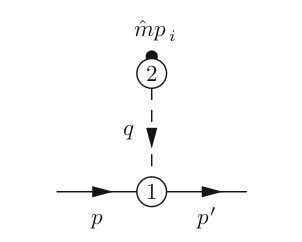
\includegraphics[scale=0.4]{pspin.png}
\end{figure}
其中赝标场与$\pi$的耦合由下面的拉式量给出
\begin{align}
   \mL_{\text{ext}}=\mbox{i}\frac{F^2B}{2}\text{Tr}(pU^{\dagger}-Up)=2BFp_i\phi_i+\cdots,
\end{align}
而$\pi NN$三点相互作用顶点由(\ref{lpin})给出,展开后可以得到
\begin{align}
   \mL_{\text{int}}=-\frac{1}{2}\frac{\mathrm{g}_A}{F}\bar{\Psi}\gamma^{\mu}\gamma_5\partial_{\mu}\phi_j\tau_j\Psi.
\end{align}

因此,对于进入的$\pi_{i}(q)$场,费曼规则如下
\begin{align}{
   \mbox{i}\Bigl(-\frac{1}{2}\frac{\mathrm{g}_A}{F}\Bigr)\gamma^{\mu}\gamma_5\tau_j\delta_{ji}(-\mbox{i}q_{\mu})}=-\frac{1}{2}\frac{\mathrm{g}_A}{F}\slashed{q}\gamma_5\tau_i.
\end{align}

最后图的结果为
\begin{align}
   \hat{m}2BF\frac{\mbox{i}}{t-M^2}\bar{u}(p^{\prime})\Bigl(-\frac{1}{2}\frac{\mathrm{g}_A}{F}\slashed{q}\gamma_5\tau_i\Bigr)u(p)=M^2F\frac{m\mathrm{g}_A}{F}\frac{1}{M^2-t}\bar{u}(p^{\prime})\gamma_5\mbox{i}\tau_iu(p).
\end{align}

通过与(\ref{Gpin})比较可得
\begin{align}
   G_{\pi N}(t)=\frac{m}{F}\mathrm{g}_A.
\end{align}
一般情况下我们定义$\pi-N$的耦合常数为
\begin{align}
   g_{\pi N}=G_{\pi N}(M_{\pi}^2)=\frac{m}{F}\mathrm{g}_A,
\end{align}
上式即著名的Goldberger-Treiman关系。


\subsection{$\pi N$散射}


考虑最低阶的$\pi N$耦合,并且假设没有外场$l_{\mu}=r_{\mu}=v_{\mu}^{(s)}=0$,因此有
\begin{align}
   \Gamma_{\mu}=\frac{1}{2}(u^{\dagger\partial_{\mu}u+u\partial_{\mu}}u^{\dagger}),\ u_{\mu}=\mbox{i}(u^{\dagger}\partial_{\mu}u-u\partial_{\mu}u^{\dagger}).
\end{align}
接着同样对$u$进行展开,我们可以得到
\begin{align}
   \mL_{\pi N N}^{(1)}=-\frac{\mathrm{g_A}}{2F}\bar{\Psi}\gamma^{\mu}\gamma_5\partial_{\mu}\phi_a\tau_a \Psi,\\
   \mL_{\pi\pi N N}^{(1)}=-\frac{1}{4F^2}\epsilon_{abc}\bar{\Psi}\gamma^{\mu}\phi_a\partial_{\mu}\phi_b\tau_c \Psi.
\end{align}
其中第一项表示赝矢型相互作用,而第二项表示接触相互作用。

从上面的拉氏量中,我们可以得到如下的费曼规则:
\begin{enumerate}
   \item 在三点相互作用中,对于入射的$\pi_a(q)$,则写下$-\frac{1}{2}\frac{\mathrm{g_A}}{F}\slashed{q}\gamma_5\tau_a$
   \item 在接触相互作用中,入射$\pi_a(q)$,出射$\pi_b(q^{\prime})$,则可以写下
   \begin{align}
      \mbox{i}\Bigl(-\frac{1}{4F^2}\Bigr)\gamma^{\mu}\epsilon_{cde}[\delta_{da}\delta_{eb}\mbox{i}q^{\prime}_{\mu}+\delta_{db}\delta_{ea}(-\mbox{i}q_{\mu})]\tau_c = \frac{\slashed{q}+\slashed{q}^{\prime}}{4F^2}\epsilon_{abc}\tau_c.
   \end{align}
\end{enumerate}

在考虑$\pi N$散射的时候,我们有如下图
\begin{figure}[h]
   \centering
   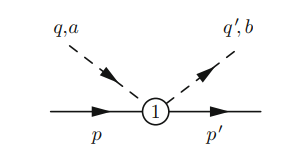
\includegraphics{pin4.png}\caption{$\pi N$接触项}
\end{figure}
\begin{figure}[h]
   \centering
   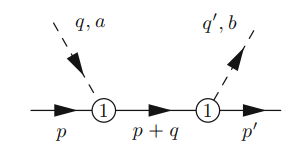
\includegraphics{pin3s.png}
   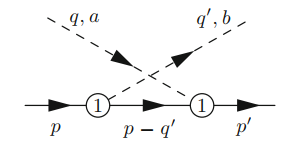
\includegraphics{pin3u.png}\caption{$\pi N$的s道和u道}
\end{figure}
因此我们的不变振幅$\mathcal{M}$有
\begin{align}
   \begin{aligned}
   \mathcal{M}_{\text{cont}}=&\bar{u}(p^{\prime})\frac{\slashed{q}+\slashed{q}^{\prime}}{4F^2}\epsilon_{abc}\tau_c u(p) = \mbox{i}\frac{1}{2F^2}\bar{u}(p^{\prime})\frac{1}{2}(\slashed{q}+\slashed{q}^{\prime})\frac{1}{2}[\tau_b,\tau_a]u(p),\\
   \mathcal{M}_{s+u}=&\mbox{i}\frac{\mathrm{g_A}^2}{4F^2}\bar{u}(p^{\prime})(-\slashed{q}^{\prime})\gamma_5\frac{1}{\slashed{p}+\slashed{q}^{\prime}-m}\slashed{q}\gamma_5\tau_b\tau_a u(p)\\
   &+\mbox{i}\frac{\mathrm{g_A}^2}{4F^2}\bar{u}(p^{\prime})\slashed{q}\gamma_5\frac{1}{\slashed{p}^{\prime}-\slashed{q}-m}(-\slashed{q}^{\prime})\gamma_5\tau_a\tau_b u(p).
   \end{aligned}
\end{align}
其中$s$和$u$道可以通过交换$a\leftrightarrow b$和$q\leftrightarrow -q^{\prime}$得到,因此我们可以只计算$s$道。
使用狄拉克方程,我们可以将$\mathcal{M}_s$化简到
\begin{align}
   \mathcal{M}_s = \mbox{i}\frac{\mathrm{g_A}^2}{4F^2}\bar{u}(p^{\prime})[(-\slashed{q}^{\prime})+4m^2\gamma_5\frac{1}{\slashed{p}^{\prime}+\slashed{q}^{\prime}-m}\gamma_5+2m]\tau_b\tau_a u(p)
\end{align}
在最低阶的树图水平上,我们可以做$m\to m_N,\mathrm{g}_A\to g_A$替换,利用
\begin{align}
   s-m_N^2=2m_N(v-v_B),
\end{align}
可以得到
\begin{align}
   \begin{aligned}
      \bar{u}(p^{\prime})\gamma_5\frac{1}{\slashed{p}^{\prime}+\slashed{q}^{\prime}-m_N}\gamma_5u(p)=&\bar{u}(p^{\prime})\gamma_5\frac{\slashed{p}^{\prime}+\slashed{q}^{\prime}+m_N}{(p^{\prime}+q^{\prime})^2-m_N^2}\gamma_5 u(p)\\
      =&\frac{1}{2m_N(v-v_B)}\Bigl[-\frac{1}{2}\bar{u}(p^{\prime}(\slashed{q}+\slashed{q}^{\prime})u(p))\Bigr],
   \end{aligned}
\end{align}
其中
\begin{align}
   \begin{aligned}
      v=&\frac{s-u}{4m_N}=\frac{(p+p^{\prime}\cdot q^{\prime})}{2m_N},\\
      v_B=&-\frac{q\cdot q^{\prime}}{2m_N}=\frac{t-2M_{\pi}^2}{4m_N}.
   \end{aligned}
\end{align}
最后我们得到s道极点的贡献
\begin{align}
   \mathcal{M}_s=\mbox{i}\frac{g_A^2}{4F_{\pi}^2}\bar{u}(p^{\prime})\Bigl[2m_N+\frac{1}{2}(\slashed{q}+\slashed{q}^{\prime})\Bigl(-1-\frac{2m_N}{v-v_B}\Bigr)\Bigr]\tau_b \tau_a u(p).
\end{align}
做$a\leftrightarrow b,q\leftrightarrow -q^{\prime}$替换后,我们可以直接得到u道的结果
\begin{align}
   \mathcal{M}_u = \mbox{i}\frac{g_A^2}{4F_{\pi}^2}\bar{u}(p^{\prime})\Bigl[2m_N+\frac{1}{2}(\slashed{q}+\slashed{q}^{\prime})\Bigl(1-\frac{2m_N}{v+v_B}\Bigr)\Bigr]\tau_a \tau_b u(p).
\end{align}

除了手征之外,我们简单介绍一下过程$\pi_a(q)+N(p)\to \pi_b(q^{\prime})+N(p^{\prime})$的$T$振幅($\mathcal{M}=\mbox{i}T$):
\begin{align}
   \begin{aligned}
   T_{ab}(p,q;p^{\prime},q^{\prime})=&\frac{1}{2}\{\tau_b,\tau_a\}T^{+}(p,q;p^{\prime},q^{\prime})+\frac{1}{2}[\tau_b,\tau_a]T^-(p,q;p^{\prime},q^{\prime})\\
   =&\delta_{ab}T^+(p,q;p^{\prime},q^{\prime})-\mbox{i}\epsilon_{abc}\tau_cT^-(p,q;p^{\prime},q^{\prime}),
   \end{aligned}
\end{align}
其中
\begin{align}
   T^{\pm}(p,q;p^{\prime},q^{\prime})=\bar{u}(p^{\prime})\Bigl[A^{\pm}(v,v_B)+\frac{1}{2}(\slashed{q}+\slashed{q}^{\prime})B^{\pm}(v,v_B)\Bigr]u(p).
\end{align}

由于$\pi\pi$具有交叉对称性
\begin{align}
   T_{ab}(p,q;p^{\prime},q^{\prime})=T_{ba}(p,-q^{\prime};p^{\prime},-q),
\end{align}
可以得到
\begin{align}
   \begin{aligned}
      A^+(-v,v_B)=&A^+(v,v_B),\ A^-(-v,v_B)=-A^-(v,v_B),\\
      B^+(-v,v_B)=&-B^+(v,v_B),\ B^-(-v,v_B)=B^-(-v,v_B).
   \end{aligned}
\end{align}

类似于$\pi\pi$散射的同位旋分解,对于$\pi N$散射,我们有
\begin{align}
   \begin{aligned}
   T^{\frac{1}{2}}=&T^++2T^-,\\
   T^{\frac{3}{2}}=&T^+-T^-.
   \end{aligned}
\end{align}
值得注意的是我们采用的$\pi^+$场和通常采用的$\pi^+$相差一个负号。

结合手征场论给出的结果,我们可以得到$A^{\pm},B^{\pm}$,绘制如表
\begin{table}[h]
   \centering
   \begin{tabular}{cccc}
      \toprule
      振幅&PV&接触项&Sum\\
      \midrule
      $A^+$&$\frac{g_A^2m_N}{F_{\pi}^2}$&0&$\frac{g_A^2m_N}{F_{\pi}^2}$\\
      $A^-$&0&0&0\\
      $B^+$&$-\frac{g_A^2}{F_{\pi}^2}\frac{m_Nv}{v^2-v_B^2}$&0&$-\frac{g_A^2}{F_{\pi}^2}\frac{m_Nv}{v^2-v_B^2}$\\
      $B^-$&$-\frac{g_A^2}{F_{\pi}^2}\frac{m_Nv_B}{v^2-v_B^2}-\frac{g_A^2}{2F_{\pi}^2}$&$\frac{1}{2F_{\pi}^2}$&$\frac{1-g_A^2}{2F_{\pi}^2}-\frac{g_A^2}{F_{\pi}^2}\frac{m_Nv}{v^2-v_B^2}$\\
      \bottomrule
   \end{tabular}
\end{table}

为了提取出散射长度,我们讨论阈值附近的动力学
\begin{align}
   v|_{\text{thr}}=M_{\pi}
\end{align}
采用归一化方式
\begin{align}
   u(p)\to \sqrt{2m_N}\binom{\chi}{0},\ \bar{u}^{\prime}\to\sqrt{2m_N}\left(\chi^{\prime \dagger} \  0\right)  
\end{align}
可以得到
\begin{align}
   T|_{\text{thr}}=2m_N\chi^{\prime\dagger}[\delta_{ab}(A^++M_{\pi}B^+)-\mbox{i}\epsilon_{abc}\tau_c(A^-+M_{\pi}B^-)]_{\text{thr}}\chi
\end{align}
代入
\begin{align}
   [v^2-v_B^2]|_{\text{thr}}=M_{\pi}^2\Bigl(1-\frac{\mu^2}{4}\Bigr),\ \mu=\frac{M_{\pi}}{m_N}=\frac{1}{7},
\end{align}
可以得到
\begin{align}
   \begin{aligned}
      T|_{\text{thr}}=&2m_N\chi^{\prime\dagger}\Bigl[\delta_{ab}\Bigl(\frac{g_A^2m_/4N}{F_{\pi}^2}+M_{\pi}\Bigl(-\frac{g_A^2}{F_{\pi}^2}\Bigr)\frac{m_N}{M_{\pi}}\frac{1}{1-\mu^2}\Bigr)\\
      &-\mbox{i}\epsilon_{abc}\tau_cM_{\pi}\Bigl[\frac{1}{2F_{\pi}^2}-\frac{g_A^2}{2F_{\pi}^2}-\frac{g_A^2}{F_{\pi}^2}\Bigl(-\frac{1}{2}\Bigr)\frac{1}{1-\mu^2/4}\Bigr]\chi.
      \Bigr]
   \end{aligned}
\end{align}

质心系中微分散射截面有
\begin{align}
   \frac{\mbox{d}\sigma}{\mbox{d}\Omega}=\frac{|\vec{q}^{\prime}|}{|\vec{q}|}\Bigl(\frac{1}{8\pi\sqrt{s}}\Bigr)^2|T|^2,
\end{align}
在开启阈处
\begin{align}
   \frac{\mbox{d}\sigma}{\mbox{d}\Omega}\mid_{\text{thr}}=\Bigl(\frac{1}{8\pi(m_N+M_{\pi})}\Bigr)^2|T|^2_{\text{thr}}=|a|^2.
\end{align}
s波散射长度被定义为
\begin{align}
   a^{\pm}_{0+}=\frac{1}{8\pi(m_N+M_{\pi})}T^{\pm}|_{\text{thr}}=\frac{1}{4\pi(1+\mu)}[A^{\pm}+M_{\pi}B^{\pm}]|_{\text{thr}},
\end{align}
下标$0+$分别表示s波和总轨道角动量。代入$A,B$的值,我们有
\begin{align}
   a_{0+}^-=&\frac{M_{\pi}}{8\pi(1+\mu)F_{\pi}^2}[1+\mO(q^2)],\\
   a_{0+}^+=&-\frac{g_A^2M_{\pi}}{16\pi(1+\mu)F_{\pi}^2}\frac{\mu}{1-\mu^2/4}\sim\mO(q^2).
\end{align}
如果代入$a^{\frac{1}{2}}=a_{0+}^++2a_{0+}^-,a^{\frac{3}{2}}=a_{0+}^+-a_{0+}^-$,则可以验证Weiberg-Tomozawa关系。
\begin{align}
   a^I=-\frac{M_{\pi}}{8\pi(1+\mu)F_{\pi}^2}\Bigl[I(I+1)-\frac{3}{4}-2\Bigr],
\end{align}
其中$I$是总同位旋。
\newpage

\renewcommand\refname{参考文献}

\bibliographystyle{unsrt}

\bibliography{ChPT}

\end{document}
